%-*- coding: UTF-8 -*-
% gougu.tex
% 勾股定理

\documentclass[UTF8]{ctexart}
\usepackage{float}

\title{杂谈勾股定理}
\author{范畴}
\date{\today}

\bibliographystyle{plain}
\begin{document}

\maketitle
\begin{abstract}
这是一篇关于勾股定理的小短文。
\end{abstract}

\tableofcontents
\section{勾股定理在古代}

西方称勾股定理为毕达哥拉斯定理,将勾股定理的发现归功于公元前 6 世纪的毕达哥拉斯学派。该学派得到了一个法则,可以求出可排成直角三角形三边的三元数组。毕达哥拉斯学派没有书面著作,该定理的严格表述和证明则见于欧几里得\footnote{欧几里得,约公元前 330--275 年。}《几何原本》的命题 47:“直角三角形些边上的正方形等于两直角边上的两个正方形之和。”证明是用面积做的。

我国《周髀算经》载商高(约公元前 12 世纪)答周公问:
\begin{quote}
\zihao{-5}\kaishu
勾广三,股修四,径隅五。
\end{quote}
又载陈子 (约公元前 7--6 世纪) 答荣方问:
\begin{quote}
\zihao{-5}\kaishu
若求邪至日者,以日下为勾,日高为股,勾股各自乘,并而开方除之,得邪以日。
\end{quote}
都较古希腊更早。
\begin{figure}[ht]
  \centering
  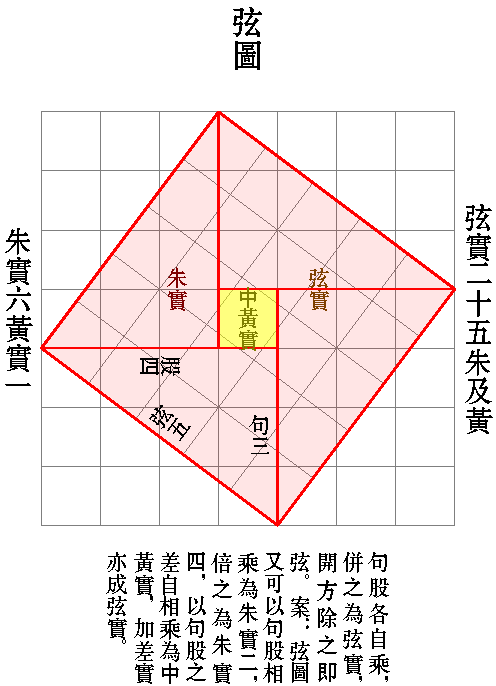
\includegraphics[scale=0.6]{xiantu.pdf}
  \caption{宋赵爽在《周髀算经》注中做的弦图(仿制),该图给出了勾股定理的一个极具对称美的证明。}
  \label{fig:xiantu}
\end{figure}

\section{勾股定理的近代形式}
\newtheorem{thm}{定理}
\begin{thm}{勾股定理}
直角三角形斜边的平方等于两腰的平方和。

可以用符号语言表述为:设直角三角形 ABC ,其中 $\angle C = 90^\circ$ ,则有
\begin{equation}
AB^2 = BC ^2 + AC^2.
\end{equation}
\end{thm}

哈哈
\begin{table}[H]
\begin{tabular}{|rrr|}
\hline
直角边 $a$ & 直角边 $b$ & 斜边 $c$ \\
\hline
	3	&		4	&		5 \\
	5	&		12 	&		13 \\
\hline 
\end{tabular}%
\qquad
($a^2 + b^2 = c^2$)
\end{table}

\bibliography{math}

\end{document}